% \documentclass[acmsmall,screen,review]{acmart} % OOPSLA
\documentclass[sigconf,review,anonymous]{acmart} % MSR

%%%%%
%% We will need to add this in camera-ready
%%%%%
%% \setcopyright{none} % to remove the copyright notice
%% \settopmatter{printacmref=false} % to remove the ACM Reference Format
%% \renewcommand\footnotetextcopyrightpermission[1]{} % to remove copyright box
\usepackage{comment}

\usepackage{lipsum}
%% \PassOptionsToPackage{hidelinks,unicode}{hyperref} % Example options

%%%%%%%%% PACKAGES

\usepackage{booktabs}     % for nice horizontal lines
%\usepackage{caption}

% --- Preamble (place in your preamble) ---
% \usepackage[switch]{lineno}
\usepackage{graphicx}
\usepackage{subcaption}
\usepackage{placeins} % for \FloatBarrier to control float placement
\usepackage{float}     % for [H] exact float placement
\usepackage{tcolorbox}
\tcbuselibrary{skins,breakable,listings}
\usepackage{listings}
\usepackage{xcolor}
\usepackage{array}
% Listings styles
\lstdefinestyle{code}{
  basicstyle=\ttfamily\small,
  numbers=left, numberstyle=\scriptsize, numbersep=6pt,
  breaklines=true, breakatwhitespace=true,
  frame=single, framerule=0.4pt,
  tabsize=2, showstringspaces=false
}
\lstdefinestyle{cpp}{style=code, language=C++}
\lstdefinestyle{json}{style=code, language=}
\lstdefinestyle{txt}{style=code, language=}

% Ensure circled step numbers in listings render reliably
% Maps Unicode circled digits to the TikZ-based \circled{n} macro
\lstset{literate=
  {❶}{{\circled{1}}}1
  {❷}{{\circled{2}}}1
  {❸}{{\circled{3}}}1
  {❹}{{\circled{4}}}1
  {❺}{{\circled{5}}}1
  {❻}{{\circled{6}}}1
  {❼}{{\circled{7}}}1
}

% A reusable “code card” environment
\newtcblisting{codecard}[2][]{%
  enhanced, breakable,
  colback=white, colframe=black!12,
  boxrule=0.6pt, arc=2mm, left=1mm, right=1mm, top=1mm, bottom=1mm,
  title={#2}, fonttitle=\bfseries\footnotesize,
  listing only, listing options={#1}
}



%% \usepackage{soul}
% xcolor is loaded by the class with the 'table' option
\usepackage{xcolor}
\usepackage{tabularx}
%% %% Custom packages end here

%% \usepackage{cite}
%% \usepackage{amsmath}
%% \usepackage{booktabs}
\usepackage{wrapfig}
\usepackage{multirow}
\usepackage{multicol}
\usepackage{enumitem}
%% \usepackage{color}
\usepackage{listings}
%% \usepackage{graphicx}
%% \usepackage{rotate}
%% %% \usepackage{url}
%% %\usepackage[hidelinks]{hyperref}
%% \usepackage{breakurl}
%% \usepackage{flushend}
\usepackage{xspace}
%% \usepackage[round-mode=places,round-precision=1,group-separator={,},group-minimum-digits={3},output-decimal-marker={.}, round-pad=false, exponent-mode = threshold, exponent-thresholds = -3:5, tight-spacing=true]{siunitx}
\usepackage{subcaption}
\usepackage{pgf-pie}
%% \usepackage{bbding}
\usepackage{pifont}
%% \usepackage{seqsplit}
%% \usepackage{pgfplots}
%% \pgfplotsset{width=7cm,compat=1.8}
%% \usepackage{datetime2}

%% % Tikz Figs
\usepackage{tikz}
\tikzset{>=latex}
%% %\usepackage{pgf-umlsd} % for flow diagram
%% \usetikzlibrary{calc}
%% \usetikzlibrary{shapes.geometric}
%% \usetikzlibrary{decorations.pathreplacing}
%% \usetikzlibrary{positioning}
\newcommand*\circled[1]{\tikz[baseline=(char.base)]{
            \node[shape=circle,draw,fill=black,text=white,inner
            sep=0.4pt] (char) {\small #1};}}

%% %%%%%%%%%% CHECKMARKS

\newcommand{\cmark}{\color{blue}{\ding{51}}}
\newcommand{\xmark}{\color{red}{\ding{55}}}

%% %%%%%%%% CONCLUDING BOXES
\usepackage[framemethod=tikz]{mdframed}
\mdfdefinestyle{mpdframe}{
   frametitlebackgroundcolor   =black!15,
    frametitlerule              =true,
    roundcorner                 =3pt,
    middlelinewidth             =1pt,
    skipabove                   =\topskip,
    skipbelow                   =\topskip,
    innermargin                 =0.1cm, % smaller makes box bigger
    outermargin                 =0.1cm,
    innerleftmargin             =0.1cm,
    innerrightmargin            =0cm,
    innertopmargin              =0.1cm,
    innerbottommargin           =0.1cm,
    align=center   
}

%%%%%%%%%% CODE and MACROS

%\input{defs-code}
%% \input{defs-logic}

%%%%%%%%%% UNCLASSIFIED
\newcommand{\Caption}[1]{\caption{#1}}
\newcommand{\NAtname}{-}
\newcommand{\specialcell}[2][c]{\begin{tabular}[#1]{@{}c@{}}#2\end{tabular}}
% Right-aligned special cell for numbers with inline deltas
\newcommand{\specialcellr}[1]{\begin{tabular}[c]{@{}r@{}}#1\end{tabular}}
\newcommand{\DefMacro}[2]{%
   \expandafter\newcommand\csname rmk-#1\endcsname{#2}%
}
\newcommand{\UseMacro}[1]{\csname rmk-#1\endcsname}


\newcommand{\YC}{\textcolor{blue}{\textbf{+}}} %{$\checkmark$}}
\newcommand{\NC}{\textcolor{red}{\textbf{-}}} %\textbf{$\times$}}}
\newcommand{\MC}{\textcolor{magenta}{\textbf{$\pm$}}}

\newcommand{\etal}{et al.}
\newcommand{\eg}{e.g.}
\newcommand{\ie}{i.e.}
\newcommand{\Fix}[1]{\textcolor{red}{[#1]}}
\newcommand{\Fixsd}[1]{\textcolor{purple}{SD:[#1]}}
\newcommand{\Mar}[1]{\textcolor{magenta}{MD:~[#1]}}
\newcommand{\Ali}[1]{\textcolor{teal}{Ali:[#1]}}
\newcommand{\Den}[1]{\textcolor{blue}{Denini:[#1]}}


\newcommand{\TODO}[1]{{\color{red}{\bf TODO:} #1}}
\newcommand{\Comment}[1]{}
\newcommand{\Boldface}[1]{\textbf{#1}}
\newcommand{\Space}[1]{}
\newcommand{\hand}[1]{\textcolor{green}{[#1]}}
\newcommand{\raw}[1]{\textcolor{red}{#1}}
\newcommand{\edit}[1]{#1}

\newcommand{\MeanStd}[2]{#1$\pm$#2}
\newcommand{\MeanStdSec}[2]{#1$\pm$#2 seconds}
\newcommand{\plus}{$+$}

\newcommand{\MyPara}[1]{\vspace{1pt}\noindent\textbf{#1}.}
\newcommand{\MyParaOnly}[1]{\noindent\textbf{#1}}
\newcommand{\MyItPara}[1]{\noindent\textit{#1}.}
\newcommand{\reducedstrut}{\vrule width 0pt height .9\ht\strutbox depth .9\dp\strutbox\relax}
%\newcommand{\InputWithSpace}[1]{\bgroup\def\arraystretch{1.1}\input{#1}\egroup}
\newcommand{\Code}[1]{{\small\ifmmode{\texttt{#1}}\else$\texttt{#1}$\fi}}
\newcommand{\CodeIn}[1]{{\small\ifmmode{\mathtt{#1}}\else$\mathtt{#1}$\fi}}
\newcommand{\ColorBack}[1]{%
  \begingroup \setlength{\fboxsep}{0pt}% \colorbox{purple!20}{\reducedstrut#1\/}% \endgroup
}

%% % ----------
%% % THIS BELOW COPIED FROM vkuncak/doc/vmcai09/defs.tex
\definecolor{gray}{RGB}{211,211,211}

%% % ----------
%% % PAPER TEXT

\newcommand{\PaperTitle}{An Empirical Analysis of Portability Issues
in Python Projects}


\newcommand{\RV}{RV\xspace}
\newcommand{\specification}{spec\xspace}
\newcommand{\specifications}{specs\xspace}
\newcommand{\Specification}{Spec\xspace}
\newcommand{\Specifications}{Specs\xspace}
\newcommand{\spec}{spec\xspace}
\newcommand{\specs}{specs\xspace}
\newcommand{\Spec}{Spec\xspace}
\newcommand{\Specs}{Specs\xspace}
\newcommand{\oss}{open-source projects\xspace}
\newcommand{\javamop}{JavaMOP\xspace}
\newcommand{\github}{GitHub\xspace}
%% \newcommand{\Tool}{\textsc{DEIMON}\xspace}
%% \newcommand{\Tool}{\textsc{DEIDMON}\xspace}
\newcommand{\x}{x\xspace}
\newcommand{\Contrib}[1]{$\star$#1}
\newcommand{\CSC}{CSC\xspace}
\newcommand{\CSCFull}{SynchronizedCollection\xspace}
\newcommand{\MUI}{MUI\xspace}
\newcommand{\MUIFull}{Map\_UnsafeIterator\xspace}
\newcommand{\STHM}{STHM\xspace}
\newcommand{\STHMFull}{StringTokenizer\_HasMoreElements\xspace}
\newcommand{\RTS}{RTS\xspace}
\newcommand{\RVTool}{RV tool\xspace}
\newcommand{\version}{revision\xspace}
\newcommand{\versions}{revisions\xspace}
\newcommand{\IMM}{IMM\xspace}
\newcommand{\IMMs}{IMMs\xspace}
\newcommand{\Isolated}{\textsc{Isolated}\xspace}
\newcommand{\NonIsolated}{\textsc{Non-Isolated}\xspace}
\newcommand{\OneUnique}{\textsc{One Unique}\xspace}
\newcommand{\MultipleUnique}{\textsc{Multiple Unique}\xspace}
\newcommand{\SingleTrace}{\textsc{Single}\xspace}
\newcommand{\Raw}{\textsc{Raw}\xspace}
\newcommand{\NoRedundant}{\textsc{No Redundant}\xspace}
\newcommand{\Sensitive}{\textsc{Sensitive}\xspace}

\newcommand{\SQ}[1]{SQ#1\xspace}
\newcommand{\SQs}{SQs\xspace}
\newcommand{\EQ}[1]{RQ#1\xspace}
\newcommand{\EQs}{RQs\xspace}

\newcommand{\sota}{SoTA\xspace}
\newcommand{\cgf}{CGF\xspace}
\newcommand{\tname}{\textsc{FlashFuzz}\xspace}
\newcommand{\acetest}{\textsc{ACETest}\xspace}
\newcommand{\ttfuzz}{\textsc{TitanFuzz}\xspace}
\newcommand{\ffuzz}{\textsc{FreeFuzz}\xspace}
\newcommand{\pathfinder}{\textsc{PathFinder}\xspace}
\newcommand{\dl}{DL\xspace}
\newcommand{\torch}{PyTorch\xspace}
\newcommand{\tf}{TensorFlow\xspace}
\newcommand{\jax}{JAX\xspace}

% Versions
\newcommand{\torchvereval}{2.2.0\xspace}
\newcommand{\tfvereval}{2.16.1\xspace}
\newcommand{\torchverwild}{2.7.0\xspace}
\newcommand{\tfverwild}{2.19.0\xspace}

% RQS OF THE PAPER
\newcommand{\RQOne}{\EQ{1}:~How prevalent are portability problems in Python projects?}

\newcommand{\RQTwo}{\EQ{2}:~What are the causes, symptoms, and fixes of portability problems?}
\newcommand{\RQTwoOne}{\EQ{2.1}: What are the root causes of portability problems in Python?}
\newcommand{\RQTwoTwo}{\EQ{2.2}: What are the symptoms of portability problems in Python?}
\newcommand{\RQTwoThree}{\EQ{2.3}: What are fix patterns for addressing portability issues?}

\newcommand{\RQThree}{\EQ{3}: How good are existing tools at detecting
and fixing portability issues?}

\newcommand{\RQFour}{\EQ{4}: How Do Developers Respond to Reported Portability Issues?}
% \newcommand{\RQFourOne}{\EQ{4.1}: What types of fixes are most commonly applied to resolve portability issues, and what solution patterns can be identified?}
% \newcommand{\RQFourTwo}{\EQ{4.2}: How do open-source developers and project communities respond to reported portability issues (issues, pull requests, or discussions)?}



% NUMBERS OF THE PAPER

% ========================================
% DATASET PARTITIONING
% ========================================
\newcommand{\NumProjectsTotal}{2{,}042}              % Total projects sampled from GitHub
\newcommand{\NumProjectsLearning}{900}                % Projects in learning set (for categorization)
\newcommand{\NumProjectsReExecution}{500}             % Projects analyzed via cross-OS test re-execution
\newcommand{\NumProjectsIssueMining}{400}             % Projects analyzed via GitHub issue mining
\newcommand{\NumProjectsApplication}{1{,}142}         % Projects in application set (for PR validation)

% ========================================
% RQ1: PREVALENCE - Test Re-execution Approach
% ========================================
\newcommand{\NumProjectsWithOSDiffInTests}{56}        % Projects with at least one test showing OS differences
\newcommand{\NumTestsExecuted}{440,728}               % Total number of test cases executed across all OSes
\newcommand{\NumTestRunsWithOSDiff}{9,508}            % Test runs showing divergent outcomes across OSes
\newcommand{\PercentDiscrepantTests}{2.16\%}          % Percentage of tests with OS differences
\newcommand{\PercentProjectsWithPortabilityReExecution}{11.2\%}  % Percentage of projects with portability issues

% ========================================
% RQ1: PREVALENCE - Issue Mining Approach
% ========================================
\newcommand{\NumIssuesMined}{2,617}                   % Total GitHub issues mined using keyword search
\newcommand{\NumIssuesAnalyzed}{240}                  % Issues manually analyzed for relevance
\newcommand{\NumIssuesRelated}{102}                   % Issues confirmed as genuine portability problems
\newcommand{\NumProjectsWithOSDiffInIssues}{95}       % Projects with confirmed portability issues from mining

% Combined results from both approaches
\newcommand{\TotalProjectsWithPortabilityIssues}{151} % Total unique projects with portability issues (56 + 95)

% ========================================
% RQ3: LLM EVALUATION - Detection and Repair
% ========================================
\newcommand{\NumCodeUsedLLM}{90}                      % Total code snippets used for LLM evaluation
\newcommand{\NumCodeNonPortableByLLM}{30}             % Non-portable snippets with OS-specific issues
\newcommand{\NumCodePortableIssue}{30}                % Portable snippets (fixed versions from issues)
\newcommand{\NumCodePortableManual}{30}               % Portable snippets (manually categorized as unrelated)

% ========================================
% RQ4: PULL REQUEST STATISTICS
% ========================================
\newcommand{\TotalPROpened}{33}
\newcommand{\TotalPRAccepted}{16}
\newcommand{\TotalPRRejected}{0}
\newcommand{\TotalPRInTestsCode}{17}
\newcommand{\TotalPRInProgramCode}{10}
\newcommand{\TotalPRInBothCode}{6}


%% Custom Macros Start Here

% Define the TODO command with highlight and margin note
\newcommand{\todo}[2][normal]{%
  \ifdefined\showtodos
    \ifstrequal{#1}{high}{\sethlcolor{red}}{}%
    \ifstrequal{#1}{normal}{\sethlcolor{yellow}}{}%
    \ifstrequal{#1}{low}{\sethlcolor{green}}{}%
    {\hl{\textbf{TODO:} #2}}%
    \marginpar{\textcolor{red}{\textbf{TODO}}}%
  \fi
}

% Control visibility of TODOs with this toggle
\newif\ifshowtodos
\showtodostrue  % Set to \showtodosfalse before final submission








%% Custom Macros End Here




\DefMacro{eq-single-performance}{\EQ{1}}
\DefMacro{eq-single-safety}{\EQ{2}}
\DefMacro{eq-evolution-stability}{\EQ{3}}
\DefMacro{eq-evolution-performance}{\EQ{4}}
\DefMacro{eq-evolution-safety}{\EQ{5}}
\DefMacro{Category}{Category}
\DefMacro{PolicyType}{Policy Type}
\DefMacro{Description}{Description}

\newenvironment{packed_itemize}{
\vspace{-0.1ex}
\begin{list}{\labelitemi}{\leftmargin=1.7em}
 \setlength{\itemsep}{0pt} \setlength{\parskip}{0pt} \setlength{\parsep}{0pt} \setlength{\headsep}{0pt} \setlength{\topskip}{0pt} \setlength{\topmargin}{0pt} \setlength{\topsep}{0pt} \setlength{\partopsep}{0pt}
 }{\end{list}
\vspace{-0.1ex}
}

\newenvironment{packed_enumerate}{
\vspace{-0.7ex}
\begin{enumerate}[label=\arabic*.,leftmargin=1.7em]%{\leftmargin=0.5em}
 \setlength{\itemsep}{0.7pt}
 \setlength{\parskip}{0pt}
 \setlength{\parsep}{0pt}
 \setlength{\headsep}{0pt}
 \setlength{\topskip}{0pt}
 \setlength{\topmargin}{0pt}
 \setlength{\topsep}{0pt}
 \setlength{\partopsep}{0pt}
}{\end{enumerate}
\vspace{-0.7ex}
}

%% This setting changes the "look-and-feel" of the paper. I don't
%% think it is a good idea to do that (not part of recommendations in
%% the CFP).  -Marcelo
%% \usepackage{draftwatermark}
%% \SetWatermarkText{DRAFT}
%% \SetWatermarkScale{1}
%% \SetWatermarkColor[gray]{0.95}
\definecolor{SubtleColor}{rgb}{0,0,.50}
\newcommand{\NA}[1]{\textcolor{SubtleColor}{ {\tiny \bf ($\star$)} #1}}

% % PyTorch Coverage Macros
% \newcommand{\torchCovPvalueAce}{0.0000}
% \newcommand{\torchCovCohenAce}{0.881}
% \newcommand{\torchCovPvaluePathfinder}{0.5805} % Keeping old value, new ones are more specific
% \newcommand{\torchCovPvaluePathfinderMinus}{0.4472}
% \newcommand{\torchCovCohenPathfinderMinus}{-}
% \newcommand{\torchCovPvaluePathfinderPlus}{0.0000}
% \newcommand{\torchCovCohenPathfinderPlus}{1.469}
% \newcommand{\torchCovPvalueTT}{0.0000}
% \newcommand{\torchCovCohenTT}{1.349}

% % TensorFlow Coverage Macros
% \newcommand{\tfCovPvalueAce}{0.0000}
% \newcommand{\tfCovCohenAce}{0.950}
% \newcommand{\tfCovPvaluePathfinder}{0.0000}
% \newcommand{\tfCovCohenPathfinder}{$-$0.612}
% \newcommand{\tfCovPvalueTT}{0.2223}
% \newcommand{\tfCovCohenTT}{0.310}

% % PyTorch Validity Ratio Macros
% \newcommand{\torchVRPvalueAce}{0.8594}
% \newcommand{\torchVRPvaluePathfinder}{0.0000}
% \newcommand{\torchVRCohenPathfinder}{0.862}
% \newcommand{\torchVRPvalueTT}{0.0000}
% \newcommand{\torchVRCohenTT}{0.536}

% % TensorFlow Validity Ratio Macros
% \newcommand{\tfVRPvalueAce}{0.0004}
% \newcommand{\tfVRCohenAce}{0.670}
% \newcommand{\tfVRPvaluePathfinder}{0.0018}
% \newcommand{\tfVRCohenPathfinder}{0.308}
% \newcommand{\tfVRPvalueTT}{0.0000}
% \newcommand{\tfVRCohenTT}{2.138}


% ------------------------------------------------------------------
% Aggregated Valid Input Generation Gains (overall)
% Minimum and maximum times higher valid-input counts for \tname vs. baselines
\newcommand{\validCountGainMin}{2.5}
\newcommand{\validCountGainMax}{1,271.3}

% TensorFlow Validity Ratio Gains (x higher)
% Range of "x" improvement in validity ratio for \tname on \tf
\newcommand{\tfValidRatioGainMin}{2.5}
\newcommand{\tfValidRatioGainMax}{5.4}

% ------------------------------------------------------------------
% RQ1 Table Delta Formatting and Values
% Usage: \deltax{\<framework>Delta<Metric><Baseline>}
% Example: \deltax{\torchDeltaTotalAce} -> (Δ 17.1×)
\newcommand{\deltax}[1]{(~#1$\times$)}

% PyTorch (\torch) deltas
\newcommand{\torchDeltaTotalAce}{17.1}
\newcommand{\torchDeltaTotalPathfinder}{4.6}
\newcommand{\torchDeltaTotalTT}{1182.0}

\newcommand{\torchDeltaValidAce}{21.3}
\newcommand{\torchDeltaValidPathfinder}{4.7}
\newcommand{\torchDeltaValidTT}{1271.3}

\newcommand{\torchDeltaRatioAce}{1.3}
\newcommand{\torchDeltaRatioPathfinder}{1.0}
\newcommand{\torchDeltaRatioTT}{1.1}

% TensorFlow (\tf) deltas
\newcommand{\tfDeltaTotalAce}{1.0}
\newcommand{\tfDeltaTotalPathfinder}{1.7}
\newcommand{\tfDeltaTotalTT}{535.3}

\newcommand{\tfDeltaValidAce}{2.5}
\newcommand{\tfDeltaValidPathfinder}{9.1}
\newcommand{\tfDeltaValidTT}{909.2}

\newcommand{\tfDeltaRatioAce}{2.5}
\newcommand{\tfDeltaRatioPathfinder}{5.4}
\newcommand{\tfDeltaRatioTT}{1.7}

\newcommand{\torchDeltaCoverageAce}{1.36}
\newcommand{\torchDeltaCoveragePathfinder}{1.52}
\newcommand{\torchDeltaCoverageTT}{1.53}

% lstsetting for python code

\lstset{language=Python,
    basicstyle=\scriptsize\ttfamily,
    keywordstyle=\color{blue}\bfseries,
    stringstyle=\color{red},
    commentstyle=\color{green!50!black}\itshape,
    morecomment=[l][\color{magenta}]{\#},
    numbers=left,
    numberstyle=\tiny,
    stepnumber=1,
    numbersep=5pt,
    showstringspaces=false,
    breaklines=true,
    frame=single,
    tabsize=2,
    captionpos=b,
    morekeywords={self, None, True, False, torch, tf, jax, float32, int32, int64, float64, uint8, uint16, uint32, uint64, complex64, complex128}
}

% coverage
\newcommand{\covtorchffvsace}{136.32\%}
\newcommand{\covtorchffvspf}{152.78\%}
\newcommand{\covtorchffvstt}{153.12\%}
\newcommand{\covtfffvsace}{102.70\%}
\newcommand{\covtfffvspf}{212.88\%}
\newcommand{\covtfffvstt}{101.13\%}

% Define colors for fix patterns (used only in Table~\ref{tab:symptoms})
\definecolor{DefensiveColor}{RGB}{65,105,225}      % blue
\definecolor{PortableColor}{RGB}{34,139,34}        % green
\definecolor{NormColor}{RGB}{205,92,92}            % red
\definecolor{EnvColor}{RGB}{138,43,226}            % violet

% Commands for colored fix patterns (used only in Table~\ref{tab:symptoms})
\newcommand{\DefensivePattern}{\textcolor{DefensiveColor}{\textbf{Defensive checks}}}
\newcommand{\PortablePattern}{\textcolor{PortableColor}{\textbf{Portable APIs}}}
\newcommand{\NormPattern}{\textcolor{NormColor}{\textbf{Normalization}}}
\newcommand{\EnvPattern}{\textcolor{EnvColor}{\textbf{Environment handling}}}


%% add page numbers
\pagestyle{plain}

\begin{document}

\title{\PaperTitle{}}

\begin{abstract}
  \sloppy
Python is broadly used across operating systems, but our cross-OS test re-execution reveals persistent portability issues. We study \NumProjects{} repositories (currently \NumProjectsAnalyzed{} projects analyzed), execute 440{,}728 tests across operating systems, and observe 9{,}508 tests with divergent outcomes; 2{,}421 differences have been analyzed so far. We identify 7 actionable root-cause categories (e.g., unavailable \texttt{os.*} methods on Windows, terminal/GUI capability gaps in CI, path/line-ending mismatches, dynamic loading issues) and curate concrete repair patterns (e.g., guards and fallbacks, cross-platform APIs, normalization). These results provide early empirical evidence of the prevalence, causes, and fix patterns of Python portability issues and establish baselines for future tools and guidelines.  
\end{abstract}

\begin{CCSXML}
<ccs2012>
   <concept>
       <concept_id>10011007.10011074.10011099</concept_id>
       <concept_desc>Software and its engineering~Software verification and validation</concept_desc>
       <concept_significance>500</concept_significance>
   </concept>
   <concept>
       <concept_id>10011007.10010940.10010992.10010993.10010994</concept_id>
       <concept_desc>Software and its engineering~Functionality</concept_desc>
       <concept_significance>500</concept_significance>
   </concept>
</ccs2012>
\end{CCSXML}

\ccsdesc[500]{Software and its engineering~Software verification and validation}
\ccsdesc[500]{Software and its engineering~Functionality}

\keywords{Mining Software Repositories, Python, Cross-Platform, Portability, Test Re-execution, Repair Patterns}

\maketitle


\section{Introduction}
\label{sec:intro}
\label{sec:sources}


A \emph{portability issue} refers to an observable difference in a
program’s behavior that arises from variations in the underlying
platform—for example, inconsistencies in API implementations or
platform-specific functionality. Python is widely regarded as a
cross-platform language, powering applications across diverse domains
such as data science, web development, and automation. It consistently
ranks among the most popular programming languages
today~\cite{stackoverflow2025,githuboctoverse2024,pypl2025}. However,
platform portability is not guaranteed. Mince et al.~\cite{mince2023},
for instance, reported that roughly 40\% of the functionality in
popular machine learning libraries (\eg{}, JAX, PyTorch, TensorFlow)
behaves inconsistently across hardware platforms such as CPUs and
TPUs. Similar challenges occur at the operating-system level; for
example, the function \CodeIn{os.geteuid()} is unavailable in Windows
distributions of Python.

Non-portable code is a significant problem: it leads to failed
deployments and reduces developer
productivity~\cite{mince2023,kiuwancodeportability,peng2024,job2024}. Although
container technologies such as Docker and Singularity/Apptainer can
mitigate these issues, most open-source Python projects are not
containerized. In our analysis of \NumProjects\ \github\ repositories,
only 19.9\% included Dockerfile or Docker compose configuration.

%% A \emph{portability issue} is an observable difference in the
%% execution of a project caused by the underlying platform, \eg{},
%% differences in API implementations that are API specific. Python is
%% widely regarded as cross-platform, powering applications from diverse
%% domains (e.g., data science pipelines, web applications, etc.) and
%% consistently ranks among the most popular programming languages of
%% today~\cite{stackoverflow2025,githuboctoverse2024,pypl2025}. Yet,
%% platform portability is not a guarantee. For example, Mince
%% \etal{}~\cite{mince2023} found that 40\% of the functionality from ML
%% Python libraries (\eg{}, \jax, \torch, and \tf) does not perform
%% consistently across different hardware (\eg{}, CPU and TPU). Similar
%% problem exists at the OS level.  For example, the Python function
%% \texttt{os.geteuid()} is unavailable on Python distributions for
%% Windows. Non-portable code is an important problem; it results in
%% failed deployments and disrupts develpment
%% productivity. Container
%% technology (e.g., Docker and Singularity/Apptainer) can mitigate this
%% problem but we find that most open source projects are not
%% containerized, i.e., they lack Dockerfiles or Singularity recipes to
%% create images. Only 19.9\% of \NumProjects{} \github projects in
%% Python we analyze contain Dockerfile or Docker compose configurations.

%% While
%% Python's design philosophy emphasizes portability through standardized
%% interfaces in modules like \texttt{os}~\cite{pymotwos,geeksos2025},
%% real-world codebases routinely contain platform-specific assumptions
%% that render them fragile across operating systems.
%% (e.g., broken
%% continuous integration, increased maintenance overhead, and broader
%% implications like 
%% These failures manifest in
%% predictable ways: missing system calls on Windows
%% (e.g., \texttt{os.geteuid()}) \cite{pythonos315}, GUI-dependent code
%% failing in headless environments, filesystem path incompatibilities,
%% and dynamic library loading issues that vary by
%% platform \Fix{Cite}. What appears to be a language-level guarantee of
%% portability dissolves under the weight of actual usage patterns and
%% environmental dependencies~\cite{peng2024,job2024}.


%%% This is way too long (distracting) to add in an introduction.
%%%
%% Our analysis of \NumProjects{} Python projects reveals significant insights regarding containerization adoption in the open-source ecosystem. Among these projects, only 345 utilize Docker through either Dockerfiles or Docker Compose configurations, representing approximately 16.9\% of the total dataset. This relatively low adoption rate highlights a critical concern: the vast majority of Python projects (83.1\%) remain potentially vulnerable to portability issues. Projects without containerization face inherent challenges in maintaining consistent execution environments across different systems, dependency management complications, and deployment reproducibility problems. The absence of Docker containerization means that these projects rely heavily on local environment configurations, Python version compatibility, and system-specific dependencies, which can lead to the infamous ``it works on my machine'' syndrome. This portability gap becomes particularly problematic when projects need to be deployed across different operating systems, cloud platforms, or when team members work with varying development setups, ultimately hindering collaboration and increasing the likelihood of environment-related bugs and deployment failures.

%% This fragility is not merely a theoretical concern. Modern software
%% development increasingly relies on cross-platform deployment, from
%% containerized applications that must run consistently across
%% different host systems to open-source projects that serve diverse
%% user communities. When portability breaks, it creates cascading
%% problems: delayed releases, increased maintenance burden, and
%% reduced software accessibility.


This paper presents a study of portability issues in Python
projects. Specifically, we analyze the prevalence of such issues,
their characteristics (e.g., symptoms, root causes, and fixes), the
effectiveness of existing tools (e.g., static analyzers and large
language models) in detecting and repairing them, and developers’
reactions to the pull requests we submitted to address portability
issues in their code. We conclude with a set of lessons we learn.
\Mar{Revise this!  $\rightarrow$} Our analysis reveals that these
portability failures, while widespread, are not chaotic or
unpredictable. Instead, they cluster around a small set of
well-defined categories—path handling, character encoding,
platform-specific APIs, and environment assumptions. Results indicate
that a combination of test re-execution and LLMs can complementary
detect issues and that LLMs can further precisely repair the issues.

This paper makes the following contributions:
\begin{packed_itemize}
  \item[\Contrib] A study about the prevalence of portability issues that use
    two complementary methods to identify issues: test re-execution
    and mining of issues with subsequent manual analysis;
  \item[\Contrib] A detailed categorization of symptoms, root causes, and fix
    patterns of portability issues;
  \item[\Contrib] An evaluation of the ability of existing tools to detect and
    repair portabi
    lity issues;
  \item[\Contrib] An evaluation about the reaction of developers about the pull
    requests we open to fix portability issues in their
    \github\ projects;
  \item[\Contrib] A dataset of \Fix{xxx} portability issues across \Fix{yyy}
    Python projects.
\end{packed_itemize}

\section{Projects and Questions}
\label{sec:methodology}

\Fix{Please review this paragraph}
This section describes the projects we used (\ref{sec:projects}), 
the setup and methodology of our experiments (\ref{sec:methods}), 
and the research questions we posed (\ref{sec:questions}).

\subsection{Projects}
\label{sec:projects}

\textbf{Dataset.} We sampled \NumProjects{} Python repositories; the analyses reported here reflect the first \NumProjectsAnalyzed{} analyzed.  
\textbf{Selection criteria.} We selected projects using \github{}'s REST API, focusing on repositories primarily implemented in Python that show evidence of testing activity (e.g., use of pytest or unittest), have at least one star, and contain at least one test case that can be executed successfully. This filtering ensures that the analyzed projects are active, testable, and representative of real-world Python software.
% i) \textbf{Language:} Python as primary language; ii) \textbf{Activity:} at least 100 commits and 10 contributors; iii) \textbf{Testing:} presence of an automated test suite (e.g., pytest, unittest); iv) \textbf{Popularity:} at least 50 stars on \github{}; v) \textbf{Diversity:} a mix of application domains (web, data science, utilities, etc.); vi) \textbf{Non-containerized:} absence of Dockerfile or Singularity recipe to create images.

\begin{table}[H]

\centering
\caption{Stats on \NumProjects{} evaluated projects: no. of tests (\#Tests), size (SLOC), no. of commits (\#Sha), age in years (Age), no. of \github{} stars ($\star$).\label{tab:project-stats}}
\begin{tabular}{lrrrrr}
\hline
Statistic & \#Tests & SLOC & \#Sha & Age & $\star$ \\
\hline
Mean & 583.94 & 42,467.26 & 2,883.25 & 6.24 & 6,147.88 \\
Median & 72 & 7,478 & 426.50 & 5.87 & 83.50 \\
Min & 1 & 2 & 2 & 0.3 & 2 \\
Max & 36,588 & 3,237,895 & 194,153 & 17.27 & 366,472 \\
Sum & 1,169,056 & 85,019,457 & - & - & - \\
\hline
\end{tabular}
\end{table}


Table~\ref{tab:project-stats} summarizes key characteristics of the
\NumProjects{} evaluated projects.  On average, each project comprises
approximately 584 tests and 42K lines of Python code (SLOC), with a
median of 72 tests and 7.5K SLOC, indicating a distribution skewed by
a few very large systems. Regarding repository activity, projects have
on average 2.9K commits, a median of 427, and span a mean lifetime of
6.2 years. The number of \github{} stars varies widely, with an
average of 6.1K, a median of only 84, and a maximum exceeding 366K,
reflecting the presence of both niche and highly popular projects.

Overall, the dataset covers a diverse range of software systems, from
small-scale repositories with only a handful of commits to large,
long-lived, and widely adopted projects.


\subsection{Research Questions and Methodology}
\label{sec:questions}

We aim to answer the following key research questions:

\sloppy \MyPara{\RQOne{}}~This question aims to assess how frequently
portability problems occur in practice. If such issues are very rare,
or if developers generally disregard them, the study’s practical value
would be limited. To address this question, we analyze issue reports
and execute tests in the wild across multiple virtual machines.
%% Although
%% Python is advertised as a cross-platform language, our preliminary
%% results suggest that many tests fail when run on different operating
%% systems. By quantifying the frequency of such issues across a
%% representative set of projects and applying statistical tests, we can
%% provide stronger evidence on whether portability is a widespread
%% concern in the Python ecosystem or only affects a small subset of
%% projects.


% \textbf{Methodology.} \Fix{Describe here the methodology to answer RQ1.}

\MyPara{\RQTwo{}}~\textbf{Rationale.}~Assuming that identifying and
resolving portability issues is an important problem, it is also
essential to understand how these issues manifest (i.e., their
symptoms), what their root causes are, and how they are typically
repaired. For instance, automated solutions become more feasible when
a small number of recurring fix patterns can be observe

%% Assuming problem of finding and
%% fixing portability issues is important, it is also important to
%% understand manifestations (\ie{}, symptoms), the root-causes of
%% portability issues, and also how they are typically repaired. For
%% example, automated solutions are more viable when a small set of fix
%% patterns exists.
% \textbf{Rationale.} This question seeks to identify and categorize the underlying reasons why portability issues arise. Our observations indicate that differences in modules such as os, file system conventions, path handling, and environment-specific assumptions may contribute to failures. In addition, some dependencies work properly on one operating system but not on another, further aggravating the problem. Understanding these root-causes is essential not only to characterize the problem but also to guide the development of best practices and tools to prevent such issues in the future.  
% \textbf{Rationale.} Recognizing diagnostic signatures helps developers quickly triage failures and identify the underlying portability issue from test logs or CI output. While not all issues produce unique error messages, many exhibit specific, reproducible patterns that enable rapid diagnosis.
%% \noindent\textit{\RQTwoOne{}}
%% \noindent\textit{\RQTwoTwo{}}
%% \noindent\textit{\RQTwoThree{}}
% \textbf{Methodology.} \Fix{Describe here the methodology to answer RQ2}

\MyPara{\RQThree{}}~This question examines the extent to which
existing tools (e.g., static analyzers and LLMs) can detect and fix
portability problems. Re-executing test suites across different OSes
(e.g., through virtual machines) can reliably identify portability
issues, but it is limited by the ability of the existing tests to
exercise the affected code locations.

%% Static tools, including
%% linters, type checkers, CodeQL queries, and even large language
%% models, can flag certain categories of issues, such as OS-dependent
%% APIs or unsafe path handling. However, many portability issues only
%% manifest at runtime, for example due to environment assumptions,
%% platform-specific encodings, or dependency incompatibilities. To
%% complement static checks, we employ a dynamic strategy—our ``rerun''
%% approach—that executes tests across multiple operating systems to
%% reveal failures that static analysis cannot anticipate. By comparing
%% the coverage of static and dynamic techniques, we can assess their
%% effectiveness and identify opportunities for improving tool support in
%% cross-platform Python development.
% \textbf{Methodology.} \Fix{Describe here the methodology to answer RQ3}


\MyPara{\RQFour{}}~This question aims to further understand technical
and social dimensions of portability issues, namely what are the
common fixes developers employ and how developers react to pull
request we submit to fix portability issues in their projects.

%% \noindent\textit{\RQFourOne{}}
%% \noindent\textit{\RQFourTwo{}}
% \textbf{Methodology.} \Fix{Describe here the methodology to answer RQ4}



\section{Results}
\label{sec:results}
% This section presents the empirical results of our study,
% organized around the research questions (RQ1–RQ4.2).
% For each RQ, we restate the rationale, present the findings,
% and provide a concise quick answer.

This section provides answering to the posed research questions.

\subsection{\textbf{Answering} \RQOne{}}
\label{rq1}

% add here: statistics, tables, and plots showing the frequency and distribution of portability issues
% for example: Table 1 (Projects analyzed, tests executed, failures observed), Figure 1 (Distribution of failures by OS)

\begin{table}[t!]
  \centering
  \caption{\label{tab:dataset}Prevalence of portability problems.}  
  \begin{subtable}[t]{\linewidth}
    \centering
    \caption{\label{tab:dataset-a}Detected problems with test re-execution.}
    \begin{tabular}{lr}
    \toprule
%    Total number of projects mined & \NumProjects{} \\
    Total number of projects selected & \NumProjectsAnalyzed{} \\
    \hspace{2ex}Total number of projects with OS differences & \NumProjectsWithOSDiffInTests{} \\    
    Total number of tests executed & \NumTestsExecuted{} \\
    \hspace{2ex}Total number of test runs with OS differences & \NumTestRunsWithOSDiff{} \\
    %Total number of differences analyzed & 2,421 \\
    \bottomrule
    \end{tabular}
  \end{subtable}
  \vspace{1ex} % space between subtables
  \begin{subtable}[t]{\linewidth}
    \centering
    \caption{\label{tab:dataset-b}Detected problems with manual inspection.}
    \begin{tabular}{lr}
      \toprule
      Total number of issues mined & \NumIssuesMined{} \\
      Total number of issues analyzed & \NumIssuesAnalyzed{} \\
      Total number of issues related & \NumIssuesRelated{}\\
      \hspace{2ex}Total number of projects with OS differences & \NumProjectsWithOSDiffInIssues{} \\
      \bottomrule
    \end{tabular}
  \end{subtable}
\end{table}


%% \Ali{Please review updates: (smaller paragraphs, remove the 100
%%   percentage accuracy of re-execution method, add example of issue
%%   mining findings, ...)}

\subsubsection{Methods}
\label{sec:methods}

We use two complementary methods to identify portability issues: (1)
test re-execution systematically reveals behavioral differences across
platforms but it is inherently incomplete as tests may not cover
important code paths; (2) issue mining includes developer's
perspectives with discussion. We discuss them in detail.

\textbf{Cross-OS test re-execution.} For each project we run the test suite
on multiple operating systems and record divergent outcomes. We then
triage failures via logs and small code inspections, mapping each
instance to a concrete category.\Mar{Is this the first time the term
  ``category'' appears? If so, explain!!.} We execute tests on
ephemeral virtual machines provided by GitHub-hosted
runners~\cite{github_actions_runners}. Each virtual machine is
automatically provisioned with 4~CPUs and 16~GB of RAM. We implemented
a single GitHub Actions workflow (YAML) that uses a matrix strategy to
run the test-suite on Ubuntu 24.04 LTS, macOS 15, and Windows Server
2025 (each job runs in a fresh VM image). Each job installs
dependencies, runs the Python tests with
\texttt{pytest}~\cite{pytest_tool} and the \texttt{pytest-json-report}
plugin~\cite{pytest_json_report} to create JSON reports, and finally
uploads the JSON files as workflow artifacts for later analysis. This
approach ensures reproducible, parallel cross-platform testing while
GitHub manages VM provisioning and maintenance.

\textbf{Issues Mining.} To complement test-based findings, we mine
\github{} issues and pull requests. We wrote a “candidate finder”
combining multiple \emph{types} of keyword:  
(a) OS/platform indicators (e.g., Windows, Linux, macOS, specific distros/architectures),  
(b) failure/fix language (e.g., fails, error, bug, fix, workaround),  
(c) testing/CI context (pytest, CI, \github{} Actions), and  
(d) common portability causes (e.g., path separators, chmod/permissions, encodings/UTF-8, dynamic libraries like \texttt{.dll}/\texttt{.so}).  
%
We combine these keywords with ``OR'' within each type and ``AND''
across types. We searched titles, bodies, and comments, with extra
weight to title and close-proximity matches. We employ a lightweight
triage (brief summaries and negative filters for off-topic mentions)
to filter spurious results. Candidate issues were normalized into
consistent records (project, link, date, summary, compact tags like
OS=, FIX=, TEST=, CAUSE=), duplicates removed, and full text (title,
description, comments) archived for analysis.

% \Mar{HEY, this is not what you are doing. You need to explain how you
% used \github{} Actions/Cloud to create VMs for different OSes.}
%\Den{Updated: Please check/revise!}

% \Den{I don't know if it's necessary and I also don't know if the text is clear enough. Please check/revise!}
% All experiments were conducted across three operating systems to ensure compatibility. The Linux setup used an AMD EPYC 7763 64-Core Processor with 4 CPUs, 16 GB RAM, and Ubuntu 24.04 LTS.

% The macOS setup ran on an Apple M2 Pro chip (Arm64) with 5 CPU
% cores, 8 GPU cores, 16 GB RAM, and macOS 15. The Windows setup used
% an AMD EPYC 7763 64-Core Processor with 4 CPUs, 16 GB RAM, and
% Windows Server 2025.

\subsubsection{Results}

This question assesses the prevalence of portability problems in
Python projects through cross-OS test re-execution and issue mining
(Section~\ref{sec:methods}). Recall that the first method is precise
but incomplete as tests can fail to reach code locations with
portability problems. The issue mining method complements the test
re-execution method but it is costly; it requires authors to
read discussion threads associated with issues to rule out spurious
cases.

Table~\ref{tab:dataset} reports on the prevalence of portability
problems in \github{} Python projects. Table~\ref{tab:dataset-a}
details the results we obtain when re-executing test cases whereas
Table~\ref{tab:dataset-b} details the results we obtain when
inspecting issues from projects. 

Table~\ref{tab:dataset-a} shows that we re-executed test suites (see
Section~\ref{sec:methods}) from a sample of \NumProjectsAnalyzed{}
projects mined from \github. Of these, we found discrepant behavior in
\PercentProjectsWithPortabilityReExecution{} of the projects, \ie{}, projects where test suites had at least one test
manifesting OS differences. The \NumProjectsAnalyzed{} projects whose
test suites were executed included a total of \NumTestsExecuted{} test
cases. Of those, we found discrepant outcomes in
\NumTestRunsWithOSDiff{} cases, which corresponds to
\PercentDiscrepantTests{}. 
%% , due to the 
%% resource-intensive nature of cross-platform test execution across
%% three operating systems.
%% Recall from Section~\ref{sec:methods} that each test suite is executed
%% on three different virtual machines and the outcomes of each test
%% cases is compared for discrepancy.

%% The test re-execution method
%% provides a systematic and reliable approach to detecting portability
%% issues by directly observing behavioral differences across
%% platforms.
%% . Due to the inherent variability of natural
%% language and the need to interpret context, we manually analyze the
%% discussion threads of the issues to confirm whether they indicate real
%% portability issues.

Table~\ref{tab:dataset-b} shows the results from mining and analyzing
\github{} issues. We mined a total of \NumIssuesMined{} candidate
issues using keyword search (see Section~\ref{sec:methods}). From this
set, we randomly sampled \NumIssuesAnalyzed{} of the most recent
issues for manual inspection. Through careful manual analysis, we
confirmed that \NumIssuesRelated{} of these were genuine portability
issues, spanning \NumProjectsWithOSDiffInIssues{} distinct
projects. Importantly, these projects have no overlap with those
analyzed in Table~\ref{tab:dataset-a}. So, we found \TotalProjectsWithPortabilityIssues{} Python projects with
portability issues.

%% \Ali{Explained where 95 distinct projects comes from.}
%% \Ali{Moved methodology discussion to RQ2 and added Table 4 showing data sources for taxonomy components.}

%\Mar{I like this discussion, but it does not belong here. The question
%is about prevalence and this text is about analysis of root causes,
%symptoms, etc. It seems to belong to the next RQs. That said, I notice
%you do not mention if the (sub)category of root cause, symptom, and
%fix originate from test re-execution or issue mining. A table showing
%(1) only re-execution, (2) only mining, (3) both with rows for the
%three cases (causes, symptom, fixes) would be ``good enough''.}


%% demonstrating that portability problems 
%% extend beyond our test execution sample and affect a broader range of 
%% the Python ecosystem.

\begin{tcolorbox}[boxrule=0pt,sharp corners,boxsep=2pt,left=2pt,right=2pt,top=2.5pt,bottom=2pt]
\textbf{RQ\textsubscript{1} (prevalence)}: We find that portability
issues are relatively prevalent. For example,
\PercentProjectsWithPortabilityReExecution{} of the
\NumProjectsAnalyzed{} projects we analyzed with cross-OS test
re-execution have portability problems.  Additionally, our issue
mining approach shows that \NumProjectsWithOSDiffInIssues{} of the
projects we analyzed have genuine portability issues.
\end{tcolorbox}

\subsection{\textbf{Answering} \RQTwo{}}

%% : test re-execution
%% (\NumTestRunsWithOSDiff{} test differences) and issue mining
%% (\NumIssuesRelated{} confirmed issues with a 42.5\% confirmation
%% rate). 
%% For instance, through issue mining we found cases\Mar{more
%%   than one?} where a project's tutorial failed on Windows due to
%% platform-incompatible dependencies, prompting maintainer discussions
%% about whether to make dependencies optional or create
%% platform-specific variants—decision-making processes and untested code
%% paths that test re-execution alone cannot
%% capture~\cite{pyearthtools-issue82}.\Mar{Can you show an excerpt of
%%   this in a listing/figure to make it more tangible?}

\subsubsection{Method}~To answer this question, we perform a
qualitative analysis about symptoms, causes, and fixes of issues.

For test re-execution, we manually inspected error messages, stack
traces, and failing test code to understand the root causes of
behavioral differences across platforms. For issue mining, we analyzed
issue titles, descriptions, developer discussions, and comments to
identify portability-related problems and their resolutions. Through
iterative open coding~\cite{strauss1990basics} across both data
sources, we identified recurring patterns and grouped instances with
similar underlying causes. This process was conducted by the authors,
with regular discussions to resolve ambiguities and refine category
definitions. The resulting taxonomy consists of \textbf{7} high-level
root-cause categories (e.g., FILE, PROC, LIB) with \textbf{24} distinct
sub-categories. For each instance, we documented observable symptoms
(error messages, behaviors) and examined corresponding fixes in merged
pull requests or commits to identify common repair
patterns. Table~\ref{tab:data_sources} summarizes the primary data
sources used to identify each component of our taxonomy. Root-cause
categories were derived from patterns observed across both test
failures and issue discussions.  Symptom signatures were primarily
extracted from test re-execution, where concrete error messages and
stack traces provide direct evidence of portability problems. Fix
patterns were identified by examining code changes and discussions in
both test-related commits and issue-related pull requests.\Mar{Can you
give summary numbers for symptoms and fixes too?}

\begin{table}[h]
\centering
\caption{Data sources for portability taxonomy components.}
\label{tab:data_sources}
\begin{tabular}{lcc}
\toprule
\textbf{Component} & \textbf{Test Re-execution} & \textbf{Issue Mining} \\
\midrule
Root-cause categories & \cmark & \cmark \\
Symptoms & \cmark & \xmark \\
Fix patterns & \cmark & \cmark \\
\bottomrule
\end{tabular}
\end{table}

In the following subsections, we elaborate on the characteristics of
 portability problems: root-causes, symptoms, and fixes.

\subsubsection{\textbf{Answering \RQTwoOne{}}}
\label{rq2-1}

~

\noindent Table~\ref{tab:categories} presents our taxonomy of portability issues 
organized by root-causes. Each row groups related sub-categories
under a main category. The columns show: (i) the root-cause category name and acronym,
(ii) specific sub-categories within that category,
(iii) a brief description of each sub-category,
(iv) the number of distinct projects where the issue appeared in test execution,
(v) the number of distinct projects where the issue appeared in mined \github{} issues, and 
(vi) the total count across both sources. 

% ========================= CATEGORIES TABLE =========================
\begin{table*}[t]
    \centering
    \caption{Taxonomy of portability issues showing root-cause categories, sub-categories, brief descriptions, and number of distinct projects observed in test execution and mined \github{} issues.}
    \label{tab:categories}
    \scriptsize
    \setlength{\tabcolsep}{3pt}
    \renewcommand{\arraystretch}{1.15}
    \begin{tabularx}{\textwidth}{
    >{\raggedright\arraybackslash}p{0.18\textwidth}
    >{\raggedright\arraybackslash}X
    >{\raggedright\arraybackslash}p{0.23\textwidth}
    >{\centering\arraybackslash}m{0.08\textwidth}
    >{\centering\arraybackslash}m{0.08\textwidth}
    >{\centering\arraybackslash}m{0.07\textwidth}
}
    \toprule
    \textbf{Root-cause category (Acronym)} & \textbf{Sub-categories} & \textbf{Description} & \textbf{\# of projects in tests } & \textbf{\# of projects in issues} & \textbf{Total} \\
    \midrule
    
    \multirow[t]{6}{*}{File and Directories (FILE)} 
    & Path separators & Forward vs. backslash differences & 7 & 27 & \multirow{6}{*}{62} \\
    & Line endings & CRLF vs. LF mismatch & 1  & 5 &                      \\
    & Case sensitivity & Filename case handling varies & 1  & 0 &                      \\
    & File locking & Windows locks open files & 7 & 4 &                      \\
    & Encoding & UTF-8 not default everywhere & 2 & 7 &                      \\
    & Filesystem block size & Block size assumptions differ & 0 & 1 &                      \\
    \midrule
    
    \multirow[t]{3}{*}{Process and Signals (PROC)}
    & Shell command execution & Shell behavior differs across OS & 5 & 14 & \multirow{3}{*}{25} \\
    & Missing signals & Signals unavailable on Windows & 3 & 2 &                      \\
    & Address already in use & Port binding conflicts vary & 1 & 0 &                      \\
    \midrule
    
    \multirow[t]{4}{*}{Library Dependencies (LIB)}
    & Platform-specific libraries (e.g. fcntl) & Unix-only libraries missing elsewhere & 2  & 1 & \multirow{4}{*}{24} \\
    & Missing libraries & Dependencies not universally available & 2 & 11 &                      \\
    & Dynamic library loading & DLL vs. SO file issues & 0 & 5 &                      \\
    & Binary wheel mismatch & Architecture-specific wheel incompatibilities & 0 & 3 &                      \\
    \midrule
    
    \multirow[t]{2}{*}{API Availability (API)}
    & Methods: os.uname(), os.geteuid(), os.getuid(), os.getpgid() & OS methods missing on Windows & 13 & 2 & \multirow{2}{*}{17} \\
    & Modules: readline, resource & Optional modules not everywhere & 0 & 2 &                      \\
    \midrule
    
    \multirow[t]{4}{*}{Environment and Display (ENV)}
    & No display in github CI (linux) & Headless CI lacks display server & 3 & 2 & \multirow{4}{*}{14} \\
    & GUI differences & Window manager behavior varies & 0 & 4 &                      \\
    & Missing curses & Curses unavailable on Windows & 1 & 0 &                      \\
    & Terminal capabilities & Terminal features differ across systems & 2 & 2 &                      \\
    \midrule
    
    \multirow[t]{3}{*}{Permissions and Limits (PERM)}
    & Permission & Permission models differ by OS & 3 & 1 & \multirow{3}{*}{7} \\
    & File descriptor limits & Resource limits vary across systems & 0 & 1 &                     \\
    & Symlink privileges & Windows requires admin for symlinks & 1 & 1 &                     \\
    \midrule
    
    \multirow[t]{2}{*}{System Information (SYS)}
    & /proc filesystem & /proc missing on macOS/Windows & 1 & 0 & \multirow{2}{*}{2} \\
    & Timezone database & Timezone data not always installed & 1 & 0 &                      \\
    \midrule
    \textbf{Total} & - & - & \textbf{\NumProjectsWithOSDiffInTests{}} & \textbf{\NumProjectsWithOSDiffInIssues{}} & \textbf{\TotalProjectsWithPortabilityIssues{}} \\
    \bottomrule
    \end{tabularx}
\end{table*}

We identify seven main root-cause categories that explain why portability problems occur:

\begin{packed_enumerate}
\item \textbf{File and Directories (FILE):} The most prevalent category (62 projects) stems
 from OS differences in file operations. Key issues include path separator differences
  (backslash vs. forward slash), line ending mismatches (\CodeIn{CRLF} vs. \CodeIn{LF}),
   file locking semantics, and text encoding defaults.

\item \textbf{Process and Signals (PROC):} This category (25 projects) captures failures
 due to OS process management differences. For example, shell execution varies across platforms
  (\CodeIn{cmd.exe} vs. \CodeIn{bash}), Windows lacks many Unix signals
   (\CodeIn{SIGHUP}, \CodeIn{SIGKILL}), and port binding produces different error codes.

\item \textbf{Library Dependencies (LIB):} These failures (24 projects) occur when code
 assumes platform-specific libraries. Issues include Unix-only modules (e.g., \CodeIn{fcntl}),
  missing dependencies, different dynamic library extensions (\CodeIn{.dll} vs \CodeIn{.so} vs
   \CodeIn{.dylib}), and architecture-specific binary wheels.

\item \textbf{API Availability (API):} This category (17 projects) covers Python APIs
 not universally available. Many OS module methods are Unix-specific (\CodeIn{os.uname()},
  \CodeIn{os.geteuid()}, \CodeIn{os.getpgid()}) and fail on Windows, while optional modules
   like readline and resource may be missing.

\item \textbf{Environment and Display (ENV):} These problems (14 projects) 
arise from runtime environment differences. Headless CI lacks display servers 
for GUI testing, window managers behave differently, terminal capabilities vary, 
and the curses module is unavailable on Windows (not included in standard Python distributions).

\item \textbf{Permissions and Limits (PERM):} These issues (7 projects) reflect OS
 differences in access control. Permission models differ (Unix chmod vs. Windows ACLs),
  file descriptor limits vary, and symbolic link creation requires admin privileges on Windows.

\item \textbf{System Information (SYS):} This category (2 projects) includes failures
 from platform-specific system information mechanisms. The /proc filesystem exists only on
  Linux, and timezone databases may not be installed by default.
\end{packed_enumerate}

\begin{figure}[!ht]
\centering
% Defensive Checks
\begin{subfigure}{0.48\textwidth}
\begin{lstlisting}[caption={Defensive check for optional library}, label={lst:defensive}]
- import readline
+ try:
+     import readline
+ except ImportError:
+     readline = None  # Fallback if readline is unavailable
\end{lstlisting}
\end{subfigure}
\hfill
% Portable APIs
\begin{subfigure}{0.48\textwidth}
\begin{lstlisting}[caption={Portable APIs: Using pathlib for cross-platform paths}, label={lst:portable}]
- import os
- home_dir = os.path.expanduser('~')
+ from pathlib import Path
+ home_dir = Path.home()  # Cross-platform home directory
\end{lstlisting}
\end{subfigure}
\vspace{0.2cm}
% Normalization
\begin{subfigure}{0.48\textwidth}
\begin{lstlisting}[caption={Normalization: Normalizing file paths}, label={lst:normalization}]
- file_path = "data/file.txt"
+ import os
+ file_path = "data" + os.path.sep + "file.txt"  # Consistent path
\end{lstlisting}
\end{subfigure}
\hfill
% Environment Handling
\begin{subfigure}{0.48\textwidth}
\begin{lstlisting}[caption={Environment handling: Using pytest skip}, label={lst:environment}]
+ import platform
+ @pytest.mark.skipif(platform.system() == "Darwin", reason="Not supported on macOS")
def test_special_case():
    ...
\end{lstlisting}
\end{subfigure}
\caption{Representative examples of fixes for portability issues: (a) Defensive checks, (b) Portable APIs, (c) Normalization, and (d) Environment handling.}
\label{fig:patterns}
\end{figure}


\subsubsection{\textbf{Answering \RQTwoTwo{}}}

\noindent\begin{table*}[t]
    \centering
    \caption{Symptom signatures and general fix patterns for portability sub-categories.
     Fix patterns are color-coded to show reuse across 
     categories: \DefensivePattern{}, \PortablePattern{}, \NormPattern{}, \EnvPattern{}.}
    \label{tab:symptoms}
    \scriptsize
    \setlength{\tabcolsep}{3pt}
    \renewcommand{\arraystretch}{1.15}
    \begin{tabularx}{\textwidth}{
        >{\raggedright\arraybackslash}m{0.06\textwidth}
        >{\raggedright\arraybackslash}m{0.18\textwidth}
        >{\raggedright\arraybackslash}X
        >{\raggedright\arraybackslash}m{0.3\textwidth}
    }
    \toprule
    \textbf{Root-cause category} & \textbf{Sub-categories} & \textbf{Symptom (verbatim error / message)} & \textbf{General Fix Pattern} \\
    \midrule
    \textbf{FILE} &
    Path separators & No specific signature & \NormPattern{} — normalize paths with pathlib \\
    & Line endings & \texttt{AssertionError: '\textbackslash r\textbackslash n' != '\textbackslash n'} & \NormPattern{} — normalize line endings \\
    & Case sensitivity & \texttt{FileNotFoundError: [Errno 2] No such file or directory: 'Readme.md'} & \NormPattern{} — case-normalize filenames \\
    & File locking & \texttt{PermissionError: [Errno 13] Permission denied: 'filename'} & \EnvPattern{} — use context managers, explicit close \\
    & Encoding & \texttt{UnicodeDecodeError: 'utf-8' codec can't decode byte 0x\{XX\} in position N: invalid start byte} & \NormPattern{} — set explicit UTF-8 encoding \\
    & Filesystem block size & No specific signature & \NormPattern{} — normalize computations avoid assumptions \\
    \midrule
    \textbf{PROC} &
    Shell command execution & No specific signature & \PortablePattern{} — use subprocess.run shell=False \\
    & Missing signals & \texttt{AttributeError: module 'signal' has no attribute 'SIGHUP'} & \DefensivePattern{} — guard signals per platform \\
    & Address already in use & \texttt{OSError: [Errno 98] Address already in use} (Linux) \; / \; \texttt{OSError: [WinError 10048] Only one usage of each socket address (protocol/network address/port) is normally permitted} (Windows) & \DefensivePattern{} + \EnvPattern{} — catch OS-specific errors, use port 0 \\
    \midrule
    \textbf{LIB} &
    Platform-specific libraries (e.g. \CodeIn{fcntl}) & \texttt{ModuleNotFoundError: No module named 'fcntl'} & \DefensivePattern{} — conditional import provide fallback \\
    & Missing libraries & \texttt{ModuleNotFoundError: No module named '...'} & \DefensivePattern{} — optional import with fallback \\
    & Dynamic library loading & \texttt{OSError: [WinError 126] The specified module could not be found} & \DefensivePattern{} — guard loading prefer pure-Python \\
    & Binary wheel mismatch & No specific signature & \EnvPattern{} — install platform-appropriate wheel \\
    \midrule
    \textbf{API} &
    Methods: os.uname(), os.geteuid(), os.getuid(), os.getpgid() &
    \texttt{AttributeError: module 'os' has no attribute 'uname'} (example) & \PortablePattern{} + \DefensivePattern{} — use platform.uname, hasattr guards \\
    & Modules: readline, resource & \texttt{ModuleNotFoundError: No module named 'readline'} (example) & \DefensivePattern{} — guard import use alternatives \\
    \midrule
    \textbf{ENV} &
    No display in github CI (linux) & \texttt{TclError: no display name and no \$DISPLAY environment variable} & \EnvPattern{} — skip GUI tests in CI \\
    & GUI differences & No specific signature & \EnvPattern{} — skip or mock GUI features \\
    & Missing curses & \texttt{ModuleNotFoundError: No module named '\_curses'} & \DefensivePattern{} — conditional import with stub fallback \\
    & Terminal capabilities & No specific signature & \EnvPattern{} — detect capabilities degrade gracefully \\
    \midrule
    \textbf{PERM} &
    Permission & \texttt{PermissionError: [Errno 13] Permission denied: '...'} & \DefensivePattern{} + \EnvPattern{} — check permissions, skip restricted tests \\
    & File descriptor limits & \texttt{OSError: [Errno 24] Too many open files} & \EnvPattern{} — close files promptly, raise limits in CI \\
    & Symlink privileges & \texttt{OSError: symbolic link privilege not held: 'src' -> 'dst'} & \EnvPattern{} — detect support and use copies \\
    \midrule
    \textbf{SYS} &
    /proc filesystem & \texttt{FileNotFoundError: [Errno 2] No such file or directory: '/proc/...'} & \PortablePattern{} — use psutil or platform APIs \\
    & Timezone database & \texttt{zoneinfo.\_common.ZoneInfoNotFoundError: 'No time zone found with key ...'} & \NormPattern{} — install tzdata or fallback \\
    \bottomrule
    \end{tabularx}
    \end{table*}   

\noindent Table~\ref{tab:symptoms} presents symptom signatures mapped to portability sub-categories.
 Each row represents a specific sub-category within a broader root-cause category (\eg{}, FILE).
  The columns show: (i) the root-cause category, (ii) the specific sub-category, (iii) verbatim error
   messages or symptoms when available, and (iv) the recommended general fix pattern. 

We find that not every sub-category produces a unique symptom signature; where concrete error messages
 exist, they reliably identify the underlying cause in test/CI logs
  (e.g., \texttt{AttributeError: module ``os'' has no attribute ``uname''},
   \texttt{UnicodeDecodeError}). These signatures enable rapid triage
    and help developers quickly recognize portability issues in practice.
 
\subsubsection{\textbf{Answering \RQTwoThree{}}}

\noindent

Figure~\ref{fig:patterns} illustrates representative examples of fix patterns
 for portability issues, drawn from real-world projects. Each subfigure demonstrates
  a different repair strategy applied to actual code. The figure shows before 
  (lines prefixed with \texttt{-}) and after (lines prefixed with \texttt{+}) 
  versions of code snippets. The four patterns demonstrated are: (a) defensive
   checks using try/except for optional imports, (b) portable APIs replacing
    OS-specific constructs with cross-platform abstractions, (c) normalization using
     path separators correctly, and (d) environment handling using platform-aware test skipping.

Across projects, portability issues are resolved through four recurring strategies:
 \textbf{(i) Defensive checks} add guards, fallbacks, \texttt{try/except}, or conditional 
 imports to handle missing APIs or modules gracefully (Listing~\ref{lst:defensive});
  \textbf{(ii) Portable APIs} replace OS-specific constructs with cross-platform abstractions
   like \texttt{pathlib}, \texttt{platform}, or \texttt{psutil} (Listing~\ref{lst:portable});
    \textbf{(iii) Normalization} standardizes encodings, line endings, paths, or filenames to
     prevent spurious differences (Listing~\ref{lst:normalization}); and \textbf{(iv) Environment handling} adapts
      code and tests to runtime conditions, such as skipping GUI tests in headless CI or
       managing platform-specific permissions (Listing~\ref{lst:environment}). 

Table~\ref{tab:symptoms} (in RQ2.2) maps each root-cause sub-category to its recommended fix pattern, showing how these four general strategies apply across the taxonomy. Figure~\ref{fig:fix_pattern_distribution} shows the distribution of these patterns, revealing that Defensive checks and Environment handling are the most common strategies (together accounting for $\sim$67\% of fixes), while Portable APIs is used less frequently but targets specific, well-defined issues. This mapping provides developers with actionable guidance: given a specific symptom or error message, the table indicates which fix pattern to apply.

\begin{figure}[ht]
\centering
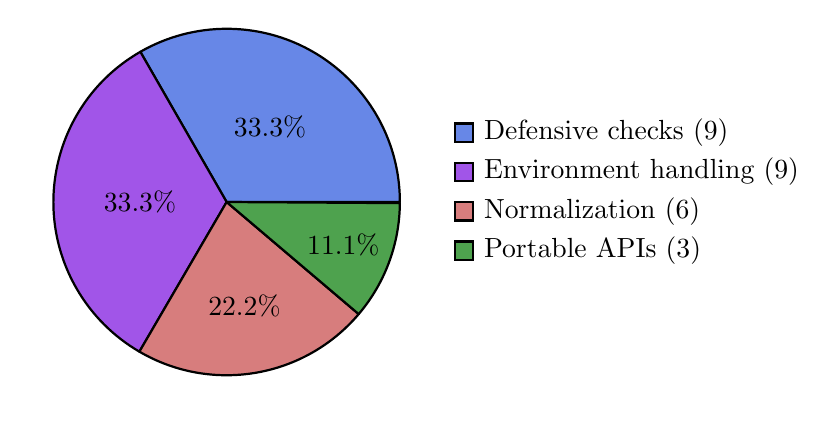
\begin{tikzpicture}
\pie[
    text=legend,
    radius=2.2,
    color={DefensiveColor!80,EnvColor!80,NormColor!80,PortableColor!80}
]{
    33.3/Defensive checks (9),
    33.3/Environment handling (9),
    22.2/Normalization (6),
    11.1/Portable APIs (3)
}
\end{tikzpicture}
\caption{Distribution of fix patterns across 24 portability sub-categories.}
\label{fig:fix_pattern_distribution}
\end{figure}

\begin{tcolorbox}[boxrule=0pt,sharp corners,boxsep=2pt,left=2pt,right=2pt,top=2.5pt,bottom=2pt]
\textbf{RQ\textsubscript{2} (characteristics)}: Portability issues cluster around 7 root-cause categories, with File and Directories (FILE) being the most prevalent (62 projects). Most issues produce distinctive error signatures that enable quick diagnosis. Four general fix patterns—defensive checks, portable APIs, normalization, and environment handling—address the majority of observed portability problems. These patterns are simple, teachable, and applicable across different categories.
\end{tcolorbox}

\subsection{\textbf{Answering} \RQThree{}}
\label{rq3}

This section evaluates performance of LLMs for detecting
(\textsection~\ref{sec:llm-detection}) and for fixing
(\textsection~\ref{sec:llm-fixing}) portability issues.

\begin{table}[t!]
\centering
  \caption{~\label{tab:llm_detection_results} LLMs for detection: metrics.}
  \vspace{-2ex}  
  \setlength{\tabcolsep}{1.5pt} % Sets the horizontal space before and after each column to 10pt
  \begin{subtable}[t]{0.5\textwidth}
    \centering
\caption{\label{tab:confusion_matrices_combined}Confusion matrices w/ 90 samples: 60 portable and 30 non-portable.}
\begin{tabular}{lccc|ccc|ccc}
  \toprule
  & \multicolumn{9}{c}{\textbf{Predicted}}\\
\cline{2-10}
& \multicolumn{3}{c|}{\texttt{llama-3.3}} &
\multicolumn{3}{c|}{\texttt{grok-4-fast}} &
\multicolumn{3}{c}{\texttt{gpt-4o-mini}} \\
\textbf{Actual} & \textbf{Port} & \textbf{NonPort} & & \textbf{Port} & \textbf{NonPort} & & \textbf{Port} & \textbf{NonPort} & \\
\midrule
\textbf{Port}     & 10 & 50 & & 53 & 7  & & 21 & 39 & \\
\textbf{NonPort}  & 4  & 26 & & 12 & 18 & & 1  & 29 & \\
\bottomrule
\end{tabular}
  \end{subtable}
  \vspace{1ex}
  \hfill
  \begin{subtable}[t]{0.5\textwidth}
    \centering
\caption{Performance metrics.}
\label{tab:llm_performance}
\begin{tabular}{lrrrrr}
\toprule
Model & Precision & Recall & F1-Score & Accuracy \\
\midrule
\texttt{llama-3.3} & 0.34 & 0.87 & 0.49 & 0.40 \\
\texttt{grok-4-fast} & 0.72 & 0.60 & 0.65 & 0.79 \\
\texttt{gpt-4o-mini} & 0.43 & 0.97 & 0.59 & 0.56 \\
\bottomrule
\end{tabular}
  \end{subtable}
\end{table}

\subsubsection{LLMs for detection}\sloppy
\label{sec:llm-detection}
\textbf{Alternative static analysis tools.} We examine the
capabilities of various popular linters for Python, namely
Ruff~\cite{ruffref}, Flake8~\cite{flake8}, Pylint~\cite{pylint},
MyPy~\cite{mypy}, Bandit~\cite{bandit}, and Pyright~\cite{pyright}.
%
We find that only Ruff provides a rule that directly addresses
potential portability concerns, namely the
\texttt{unspecified-encoding} check~\cite{encruff} that maps to the
``Encoding'' sub-category within the ``File and Directories''
category. The remaining tools focus primarily on style, type
correctness, security, and general code quality. For that reason, we
focus on LLMs. We consider three LLMs of moderate model size, namely
\texttt{llama-3.3}~\cite{llama3}, \texttt{Grok-4-Fast}~\cite{grok4},
and \texttt{GPT-4o-Mini}~\cite{gpt4o}

%% This rule helps identify cases where files are opened
%% without explicitly specifying an encoding, which may lead to
%% cross-platform inconsistencies. The remaining tools focus primarily on
%% style, type correctness, security, and general code quality, without
%% offering rules specifically designed to detect
%% operating-system-dependent behaviors or other portability issues.
%% \Den{@Marcelo, everything below is new and needs to be revised!}
%% \textbf{Motivation for LLM Evaluation.}
%% Given the limited support for portability checks in existing static
%% tools, we extended our evaluation to large language models (LLMs).

\noindent\textbf{Setup.}~We sampled a total of \NumCodeUsedLLM{} code
snippets to evaluate performance of LLM: (i)~\NumCodeNonPortableByLLM{} non-portable snippets
containing OS-specific constructs, (ii)~\NumCodePortableIssue{} portable snippets that had
been fixed by developers (mined from issues), and (iii)~\NumCodePortableManual{} code we
manually categorized as portable. This distribution attempts to
reflect a more realistic division of code seen in the wild, where
portability violations are less frequent. We used the openrouter.ai
API~\cite{openrouter} to interact with the models. Each model was
prompted with a consistent template that included the code snippet and
a question asking whether the code was portable across Windows, Linux,
and Mac. The models' responses were parsed to extract their
classification decisions.
% 
%% Unrelated code was treated as portable for classification purposes, since such snippets do not exhibit any portability problems. Consequently, the dataset comprised 60 portable samples (30 corrected + 30 unrelated) and 30 non-portable samples. 
% 

\noindent\textbf{Metrics.}~We used standard metrics in data sciences
to measure performance of binary classifiers (e.g., precision, recall,
accuracy, etc.). Table~\ref{tab:llm_detection_results} shows
results. Table~\ref{tab:confusion_matrices_combined} shows the
confusion matrices associated with each LLM, illustrating the
classification of the \NumCodeUsedLLM{} samples and
Table~\ref{tab:llm_performance} shows the metrics.

%% By comparing the models' predictions against the known classification
%% of each snippet, we quantitatively assessed their ability to identify
%% cross-platform issues. Specifically, we computed precision, recall,
%% F1-score, and accuracy for each model.
%% % 
%% These metrics provide an objective measure of how effectively LLMs can
%% detect or reason about portability issues—an area where traditional
%% static tools often fall short. This setup allows us to explore whether
%% LLMs can complement static analyzers by offering probabilistic
%% insights into potential cross-platform
%% hazards.

\noindent\textbf{Analysis of results.}~ Their results indicate a
limited ability of LLMs to accurately reason about portability
issues. llama-3.3 and GPT-4o-Mini are ``pessimistic'' and report too
many alarms, most of which are false positives. In contrast,
Grok-4-Fast is more cautious in reporting but misses lots of true
positives.
%% In practical terms, these results suggest complementary reasoning profiles across models:
%% \begin{enumerate}
%%   \item \texttt{llama-3.3}: Highly cautious and overgeneralizing reasoning—maximizes detection coverage but produces many false positives.
%%   \item \texttt{Grok-4-Fast}: Balanced reasoning—achieves the best trade-off between recall, precision, and overall accuracy.
%%   \item \texttt{GPT-4o-Mini}: Over-sensitive reasoning—detects almost all non-portable cases but lacks discrimination power.
%% \end{enumerate}


%% a tendency to rely on surface-level
%% heuristics rather than deep contextual understanding of cross-platform
%% behavior. Addressing this limitation will require more explicit
%% exposure to platform-diverse examples during instruction tuning and
%% evaluation.
%% Table~\ref{tab:confusion_matrices_combined} presents the confusion matrices for all three models evaluated. The matrices reveal distinct classification patterns across models. \texttt{Grok-4-Fast} demonstrates the most balanced performance, correctly identifying 53 out of 60 portable cases and 18 out of 30 non-portable cases, yielding an overall accuracy of 79\%. In contrast, \texttt{llama-3.3} exhibits a strong bias toward the non-portable class, misclassifying 50 of the 60 portable samples, resulting in only 40\% accuracy. \texttt{GPT-4o-Mini} shows an opposite tendency: while it achieves near-perfect specificity (29 out of 30 non-portable cases correctly identified), it misses the majority of portable cases (39 out of 60), achieving 56\% accuracy. These patterns suggest fundamentally different decision boundaries and risk tolerance levels across the three models, which we analyze in detail below.

%% The extended evaluation provides new insight into how different LLMs reason about software portability under a more diverse and balanced dataset. The inclusion of ``unrelated'' yet valid Python code introduces a subtle but important challenge: distinguishing the absence of portability issues from the presence of clear portability signals. This distinction is conceptually close to the notion of false alarms in static analysis and serves as a more realistic proxy for practical development scenarios.

%% % talking about the precision, recall, f1-score, accuracy now:

%% The \texttt{llama-3.3} model achieved the lowest precision 34\% and accuracy 40\%, while maintaining the highest recall 87\%. This means that Llama correctly identified most non-portable cases but did so with a substantial number of false alarms—frequently flagging portable code as non-portable. Its confusion matrix (Table~\ref{tab:confusion_matrices_combined}) confirms this pattern: the model displays a highly cautious bias, tending to classify almost any code snippet as potentially non-portable.
%% % 
%% This behavior reflects a risk-sensitive but shallow reasoning strategy, where the model overestimates portability issues without truly distinguishing between harmless platform-specific constructs and genuine cross-platform incompatibilities. As a result, Llama achieves strong coverage at the expense of reliability, limiting its effectiveness for precise portability assessment.

%% In contrast, \texttt{Grok-4-Fast} exhibited the most balanced and effective performance, with a precision of 72\%, recall of 60\%, F1-score of 65\%, and the highest accuracy (79\%). Its confusion matrix (Table~\ref{tab:confusion_matrices_combined}) shows that Grok successfully differentiates between portable and non-portable code in most cases, striking a reasonable balance between sensitivity and specificity.
%% %
%% The model demonstrates contextual generalization, capturing both syntactic and semantic cues related to platform-dependent constructs. However, its moderate recall suggests a cautious tendency to miss some non-portable samples, favoring correctness over exhaustive detection.

%% The \texttt{GPT-4o-Mini} model achieved the highest recall (97\%), outperforming the others in its ability to detect nearly all non-portable cases. Nevertheless, its low precision (43\%) and moderate accuracy (56\%) indicate a strong over-detection bias—GPT-4o tends to classify many portable codes as problematic.

%% This pattern reveals a highly inclusive reasoning style: the model is eager to label code as non-portable, prioritizing coverage rather than precision. Such behavior, while useful for exploratory or preventive analysis, may produce excessive false positives in practical settings where diagnostic accuracy is essential.


%% From a broader research standpoint, the findings indicate that all three models possess a functional grasp of portability-related cues—such as system-dependent paths, OS-specific APIs, and encoding assumptions—but none exhibit fine-grained semantic discrimination. 
%
%% \textbf{Answer.} \Fix{turn this into a box anwser:}Static tools
%% (linters, CodeQL, LLM prompts) can detect some issues but miss
%% runtime failures. Dynamic re-execution across OSes (our approach)
%% provides broader coverage.


\subsubsection{LLMs for fixing.}
\label{sec:llm-fixing}
\noindent\textbf{Setup.}~ Following the classification experiment, we designed a complementary evaluation focused on the corrective capabilities of LLMs. In this phase, we used the \NumCodeNonPortableByLLM{} non-portable Python snippets identified earlier and prompted each model with two distinct repair configurations.  
In the first configuration (\textit{generic prompt}), each model received a general instruction stating that the code exhibited portability issues and was asked to produce a corrected version.  
In the second configuration (\textit{pattern-guided prompt}), each non-portable snippet was accompanied by a description of the specific portability issue (derived from our taxonomy in \ref{rq2-1}) and the corresponding \textit{General Fix Pattern} from Table~\ref{tab:symptoms}.  
This design aimed to evaluate whether structured repair guidance could improve the models' ability to generate functionally portable code. Each model attempted to fix all \NumCodeNonPortableByLLM{} snippets, resulting in 90 repair attempts per configuration.

\noindent\textbf{Metrics.} ~We evaluated the correctness of each generated fix using two criteria:  
(i) the modified code must execute successfully without errors across all target platforms (Linux, macOS, Windows), and  
(ii) the fix must preserve the intended functionality of the original program.  
Fixes that met both criteria were considered \textit{correct}; otherwise, they were labeled as \textit{incorrect}.  
Accuracy was computed as the ratio of correct fixes to the total number of attempted repairs per model.

\begin{table}[t]
\centering
\caption{Performance of LLMs in generating portability fixes across both prompt configurations (\NumCodeNonPortableByLLM{} samples per model).}
\label{tab:llm_fix_results_combined}

\begin{subtable}[t]{0.47\textwidth}
\centering
\caption{Generic prompt.}
\begin{tabular}{lrrr}
\toprule
\textbf{Model} & \textbf{Correct} & \textbf{Incorrect} & \textbf{Accuracy} \\
\midrule
\texttt{grok-4-fast} & 13 & 17 & 0.43 \\
\texttt{gpt-4o-mini} & 10 & 20 & 0.33 \\
\texttt{llama-3.3} & 8 & 22 & 0.27 \\
\bottomrule
\end{tabular}
\end{subtable}
\hfill
\begin{subtable}[t]{0.47\textwidth}
\centering
\caption{Pattern-guided prompt.}
\begin{tabular}{lrrr}
\toprule
\textbf{Model} & \textbf{Correct} & \textbf{Incorrect} & \textbf{Accuracy} \\
\midrule
\texttt{grok-4-fast} & 23 & 7 & 0.77 \\
\texttt{gpt-4o-mini} & 21 & 9 & 0.70 \\
\texttt{llama-3.3} & 15 & 15 & 0.50 \\
\bottomrule
\end{tabular}
\end{subtable}
\end{table}

\noindent\textbf{Analysis of results.}~ The results in Table~\ref{tab:llm_fix_results_combined} show that all models exhibited limited success under the generic prompt setting, with accuracies ranging from 27\% to 43\%.  
This indicates that, when provided with only minimal context, most LLMs struggle to infer the exact nature of portability issues and to produce appropriate cross-platform corrections.  
While the \texttt{grok-4-fast} model outperformed the others, its success rate remained below 50\%, suggesting that general-purpose reasoning alone is insufficient for precise code repair in this domain.

In contrast, the pattern-guided configuration substantially improved repair performance across all models.  
The inclusion of explicit problem descriptions and generalized fix patterns increased accuracy by more than 30 percentage points on average.  
The \texttt{grok-4-fast} model achieved the highest accuracy (76.67\%), demonstrating a clear ability to integrate structured repair hints into its reasoning process.  
Similarly, \texttt{gpt-4o-mini} reached 70\%, producing fixes that were more consistent with the intended patterns while preserving functional correctness.  
The \texttt{llama-3.3} model also showed moderate improvement (50\%), particularly in cases involving straightforward path and API adjustments, though it still struggled with more complex logic integration.

Overall, these findings highlight the strong impact of guided contextualization on LLM-based repair.  
When supplied with explicit repair patterns, the models produced significantly more reliable and semantically consistent fixes, confirming that structured guidance can substantially enhance cross-platform reasoning capabilities in code generation tasks.

\begin{tcolorbox}[boxrule=0pt,sharp corners,boxsep=2pt,left=2pt,right=2pt,top=2.5pt,bottom=2pt]
\textbf{RQ\textsubscript{3}:} Traditional static analysis tools provide very limited support for portability issues—only Ruff includes a specific rule related to encoding. 

\textbf{For detection}, LLMs show potential over traditional tools. They achieved strong recall and precision, with the best model reaching approximately 70\%, suggesting that they can reliably identify portability-related problems in source code. 

\textbf{For repair}, however, their performance remains less limited. When prompted to fix 30 faulty snippets, success rates ranged from 33--43\% with generic prompts, increasing to 50--77\% only when explicit issue descriptions and repair patterns were provided. Overall, results indicate that while LLMs can recognize and occasionally correct portability issues, achieving reliable automated repairs still requires structured guidance or integration with static verification tools.


\end{tcolorbox}


\subsection{\textbf{Answering} \RQFour{}}
This section discusses the analysis of pull requests (PRs) submitted to open-source projects to address portability issues identified in our study.
\label{sec:pr-discussion}

%

% Add here: time-to-fix statistics, issue/PR comment analysis
% For example: Figure 4 (Distribution of time-to-fix), Table 5 (Engagement metrics per project)

\subsubsection{Methodology}
\Fix{This subsubsction is old, please update if needed.}
To validate our findings and contribute back to the open-source ecosystem, we submitted pull requests addressing the portability issues uncovered in our study. Our contributions focused on libraries where our analysis revealed systematic portability challenges, proposing fixes to improve cross-platform compatibility and robustness.

Table~\ref{tab:prs} summarizes the results of this effort. We submitted a total of \TotalPROpened{} pull requests (PRs) spanning 6 categories of portability issues, of which \TotalPRAccepted{} had been accepted at the time of writing. The overall acceptance rate of 33\%, along with a zero rejection rate, indicates that the issues we identified correspond to genuine portability problems recognized by library maintainers. Notably, ``File and Directories'' issues were the most frequent (18 PRs), reflecting the prevalence of path, encoding, and file handling inconsistencies across platforms. Conversely, ``Process and Signals'' issues exhibited the highest acceptance rate (100\%), likely due to their critical impact on application functionality.


From this number of PRs, we observe that the fix was applied in \TotalPRInTestsCode{} cases to the test code only, in \TotalPRInProgramCode{} cases to the program code only, and in \TotalPRInBothCode{} cases to both the test and program code. This distribution suggests that while some portability issues can be resolved by adjusting tests to be more environment-aware, many require changes to the application logic itself to ensure consistent behavior across platforms.

\begin{table}[h!]
    \centering
    \footnotesize
    \setlength{\tabcolsep}{2pt}
    \caption{
      % \Fix{Ali, please update this table with the latest results.} 
      Summary of Pull Requests (PRs) by issue type, showing opened, accepted, and rejected. The last row shows totals.}
    \label{tab:prs}
    % Creating a compact tabular environment
    \begin{tabular}{lccc}
        \toprule
        \textbf{Category} & \textbf{Opened} & \textbf{Accepted} & \textbf{Rejected} \\
        \midrule
        File and Directories & 18 & 6 & 0 \\
        API Availability & 12 & 2 & 0 \\
        Process and Signals & 2 & 2 & 0 \\
        System Information & 2 & 1 & 0 \\
        Library Dependencies & 1 & 1 & 0 \\
        Environment and Display & 1 & 0 & 0 \\
        \midrule
        \textbf{Total} & \textbf{\TotalPROpened} & \textbf{\TotalPRAccepted} & \textbf{\TotalPRRejected} \\
        \bottomrule
    \end{tabular}
\end{table}

% \textbf{Quick Answer.} Developers typically acknowledge portability problems but often give them lower priority than functional bugs, resulting in varied resolution times.  


\Den{The following three subsections are new. Please review.}
\subsubsection{The webassets case study}
% https://github.com/miracle2k/webassets/pull/562

We illustrate how portability issues manifest and are fixed through a case study of the webassets project~\cite{webassets}. Webassets is an asset management library for Python web development with 932 stars on GitHub, used for bundling and processing web assets like CSS and JavaScript files.

The problem we encountered falls into the \textbf{File and Directories (FILE)} category, specifically the ``File locking'' sub-category. The issue occurred in the test suite where \CodeIn{tempfile.NamedTemporaryFile} was used without disabling automatic deletion, causing failures on Windows due to platform-specific file locking behavior. On Windows, the operating system locks open files more aggressively than on Unix-like systems, preventing the same file from being reopened while still in use.

Listing~\ref{lst:webassets_fix} shows our fix applied to the test file. The original code created a temporary file within a context manager that automatically deleted the file upon exiting the \texttt{with} block. However, on Windows, attempting to reopen this file (which the test needed to do) failed because the file was still locked by the previous file handle.
 %, language=diff

\begin{lstlisting}[caption={Diff showing our approved PR for webassets temporary file handling issue.}, label={lst:webassets_fix}]
 @pytest.fixture
 def tmp_file():
-  with tempfile.NamedTemporaryFile(mode="wt") as f:
+  with tempfile.NamedTemporaryFile(mode="wt", delete=False) as f:
     for _ in range(100):
       f.write("\n")
     f.flush()
-    yield f.name
+    tmp_path = f.name  # store path before file is closed
+  yield tmp_path
+  os.remove(tmp_path)  # clean up after the test
\end{lstlisting}

Our fix addresses this issue by modifying line 4 to disable automatic deletion using \texttt{delete=False}, storing the file path on line 8 before the file handle is closed, and manually cleaning up the temporary file on line 10 after the test completes. This pattern exemplifies the \textbf{Environment handling} fix strategy from our taxonomy, where platform-specific behavior is accommodated through careful resource management.

This case demonstrates how seemingly simple operations like temporary file creation can have subtle portability implications that only manifest under specific platform conditions, highlighting the importance of cross-platform testing for robust software development.


\subsubsection{The pydantic-extra-types case study}
% https://github.com/pydantic/pydantic-extra-types/pull/333

We present another illustrative case study from the pydantic-extra-types project~\cite{pydantic_extra_types}. Pydantic-extra-types is a library that provides additional type validators for Pydantic with 290 stars on GitHub, used for extending Pydantic's validation capabilities with specialized data types.

The problem we encountered also falls into the \textbf{File and Directories (FILE)} category, specifically the ``Path separators'' sub-category. The issue occurred in test fixtures where \CodeIn{os.path.relpath} was used to create relative paths from absolute paths. On Windows, this function fails when the source and target paths are on different drives (e.g., \texttt{C:\textbackslash} vs \texttt{D:\textbackslash}), as Windows cannot create relative paths between different drive letters.

Listing~\ref{lst:pydantic_fix} shows our fix applied to three test fixtures in the \CodeIn{test\_path.py} file. The original code assumed that \CodeIn{os.path.relpath} would always succeed, but on Windows systems where temporary directories might be created on a different drive than the current working directory, this assumption breaks and causes test failures.

\begin{lstlisting}[caption={Diff showing our fix for pydantic-extra-types cross-drive relative path issue.}, label={lst:pydantic_fix}]
  @pytest.fixture
  def relative_file_path(absolute_file_path: pathlib.Path) -> pathlib.Path:
+   cwd = pathlib.Path.cwd()
+   if os.name == 'nt' and absolute_file_path.anchor != cwd.anchor:
+     # on windows, cant create relative path when paths are on different drives
+     return absolute_file_path
    return pathlib.Path(os.path.relpath(absolute_file_path, os.getcwd()))
\end{lstlisting}

Our fix addresses this Windows-specific limitation by detecting when the OS is Windows (lines 3-6) and checking whether the absolute path and current working directory have different anchors (drive letters). When this condition is met, the function returns the absolute path instead of attempting the problematic relative path conversion. This pattern exemplifies the \textbf{Environment handling} fix strategy from our taxonomy, where platform-specific limitations are accommodated through conditional logic.

This case demonstrates how path operations that work seamlessly on Unix-like systems can encounter fundamental limitations on Windows due to the multi-drive architecture, highlighting the importance of considering platform-specific filesystem constraints in cross-platform development.

% 
% OLD:
% 
% To better understand how open-source developers and project communities react when portability issues are reported, we submitted pull requests (PRs) across different projects. The responses we received illustrate a spectrum of engagement patterns, from prompt acceptance to rejection or non-merge due to project inactivity.

% \cite{breds_pr_40}
% In one case, the proposed change addressed a test portability issue arising from platform-specific file handling. The original test used Python's \texttt{tempfile.NamedTemporaryFile} without disabling automatic deletion, which led to failures on Windows due to how temporary files are closed and reopened. Our fix stored the path before closing the file and explicitly removed it after the test execution. The maintainer accepted the contribution, commenting: \emph{``Thanks for this.''}, 
% in another PR, the maintainer expressed appreciation for the contribution and promptly merged the fix, stating: \emph{``Thanks a lot for this contribution! Good catch.''}
% \cite{python_doit_api_pr_9}. 
% These responses highlight a positive and collaborative stance, where developers value external input and promptly integrate fixes that improve cross-platform compatibility.

% \cite{frequenz_pr_1261}

\subsubsection{The frequenz-sdk-python case study}
% https://github.com/frequenz-floss/frequenz-sdk-python/pull/1261

We encountered a different type of response when addressing a dependency portability issue in the frequenz-sdk-python project~\cite{frequenz_sdk_python}. Frequenz-sdk-python is an energy management SDK for Python applications. The problem we identified falls into the \textbf{System Information (SYS)} category, specifically the ``Timezone database'' sub-category.

The issue occurred in the test suite where tests relied on the \CodeIn{zoneinfo} and \CodeIn{tzdata} modules for timezone operations. These modules are not consistently available across all platforms—while \CodeIn{zoneinfo} is included in Python 3.9+ on most systems, the timezone data (\CodeIn{tzdata}) may not be installed by default on some Windows configurations. This caused test failures when the required timezone information was unavailable.

Our initial proposed solution involved conditional installation of the \CodeIn{tzdata} dependency specifically for Windows environments, following a \textbf{Defensive checks} approach by detecting the platform and installing the missing dependency when needed. However, during the discussion with the project maintainer, a different perspective emerged. The maintainer argued that rather than adding platform-specific complexity to handle the dependency, the better long-term solution was to remove the reliance on these timezone-specific modules altogether. This approach follows a \textbf{Simplification} strategy—instead of accommodating platform differences, the codebase was simplified to avoid the problematic dependency entirely. As a result, the PR was reduced to removing the timezone-dependent tests and related functionality.

This case illustrates an important aspect of how development communities approach portability issues: sometimes maintainers prefer architectural simplification over platform-specific workarounds, prioritizing code maintainability and reducing complexity rather than supporting edge cases across all possible platform configurations.

% Finally, in another project, the response was shaped less by technical considerations and more by the project's state of maintenance. The maintainer acknowledged the validity of the patch but declined to merge it, noting: \emph{``I do somewhat view that project as archived and inactive... My concern about merging is that an updated last commit date would make the project seem more active than it really is.''} This case illustrates how project activity levels and community sustainability strongly influence whether portability improvements are accepted, even if the technical changes are sound.

% Overall, these three cases demonstrate that responses to portability
% contributions vary significantly: active projects may readily adopt
% fixes, maintainers may prefer design simplifications over
% platform-specific adjustments, and inactive projects may resist
% merging altogether to avoid signaling misleading project vitality.

\section{Lessons Learned}
\label{sec:lessons}

\Den{What should developers, researchers, and tool builders keep in mind when thinking about portability issues in Python? Here are some suggestions:}
% - Practical guidelines distilled from study
% - Recommendations for writing portable Python code
% - Recommendations for tool designers and researchers
% - General lessons beyond Python (cross-platform SE insights)

% Not in a philosophical way, but in a practical way, what are the main takeaways from our study? 

% \begin{itemize}
%   \item \textbf{Portability is not automatic.} Even though Python is designed to be cross-platform, real projects still often break when run on different operating systems. Portability depends on how code and environments are actually used, not just what the language promises.
%   \item \textbf{Problems fall into repeatable categories.} The failures we found were not random. They fall into a small set of categories (like paths, encodings, missing APIs). This means we can focus research and tool support on the most common categories instead of treating each bug as unique.
% \end{itemize}

This section distills practical insights from our study for developers and researchers working with cross-platform Python code.

\noindent\textbf{Prioritize file and directory handling.}
File-related issues (FILE) were both the most common category in our taxonomy (59 instances) and the most frequent target of our pull requests (18 PRs). Path separators, line endings, encoding defaults, and file locking behavior vary significantly across platforms. Use cross-platform abstractions such as \texttt{pathlib} for paths and explicitly specify encoding when opening files. Avoid hardcoding path separators or making assumptions about filesystem case sensitivity.

\noindent\textbf{Process and signal issues are rare but critical.}
While process and signal-related problems (PROC) accounted for only 2
pull requests, they achieved a 100\% acceptance rate from
maintainers. When such issues occur, they typically have severe
functional impact—crashes, hangs, or incorrect behavior. Developers
should test subprocess invocation, signal handling, and process
management across platforms early in development, as these issues are
immediately recognized as critical by the community.

\section{Threats to Validity}
\label{sec:threats}
% - Internal validity: correctness of rerun framework
% - External validity: generalization beyond studied projects
% - Construct validity: definitions of “portability” and categorization
% - Conclusion validity: statistical soundness, possible biases

\Fix{one thing we remember is that we do not explore other versions of OSs}


\section{Related Work}
\label{sec:related}
% - Prior work on cross-platform failures, portability in SE
% - Studies on testing across operating systems
% - Tool support for detecting environment-specific issues
% - Positioning of this work relative to literature

Several lines of research have explored the detection, characterization, and mitigation of portability and reliability issues in software systems.

Pysa~\cite{pysa2021}, developed by Meta, is a static analysis framework for Python that performs data-flow tracking to identify potential security vulnerabilities. By tracing information from sources to sensitive sinks, Pysa enables early detection of flaws in large-scale codebases, reducing security risks without executing the code. Its design illustrates how static analysis can be leveraged to uncover subtle issues in dynamic languages such as Python.

Vahabzadeh \etal{}~\cite{vahabzadeh2015empirical} conducted a comprehensive empirical study on defects in test code, revealing that such bugs are both pervasive and detrimental to software quality. They report that approximately 18\% of these issues stem from environmental factors, particularly differences between Windows and Unix platforms. This finding underscores the role of environment-related faults as a major source of unreliability in testing infrastructures.

Rasley \etal{}~\cite{rasley2015detecting} introduced \CodeIn{CheckAPI}, a runtime framework for detecting latent cross-platform API violations by contrasting execution traces against platform-specific interface specifications. Their approach identifies compatibility problems that remain undetected during standard testing yet may trigger failures when software is deployed on different operating systems. This work emphasizes the importance of uncovering non-manifest portability bugs that traditional test suites often overlook.

Complementing these efforts, Ghandorh \etal{}~\cite{ghandorh2020systematic} performed a systematic literature review of metrics and methodologies for assessing software portability. Their findings highlight the fragmented nature of current research in this domain and the absence of a standardized framework for quantifying portability across systems and environments.

Finally, Sun \etal{}~\cite{sun2016bear} proposed \textit{Bear}, a framework that statistically measures application sensitivity to operating system (OS) variability. By analyzing how nondeterministic OS behaviors affect reliability and performance, they demonstrate that assumptions about OS predictability can lead to unforeseen failures. This perspective complements application-level analyses by reinforcing the need to account for environmental uncertainty in ensuring robust and portable soft



\Fix{Talk about} \cite{vahabzadeh2015empirical} here. Others: \cite{rasley2015detecting, ghandorh2020systematic}

Maybe: \cite{sun2016bear}. Mobile apps testing: \cite{boushehrinejadmoradi2015testing}

\section{Conclusions and Future Work}
\label{sec:conclusions}
% - Recap of findings for each RQ
% - Key contributions
% - Long-term impact on research and practice
% - Future directions

%% \section*{Data Availability}

%% The artifacts -- including datasets and scripts -- are publicly available~\cite{ourrepo}.

\onecolumn \begin{multicols}{2}
%\balance
\bibliographystyle{ACM-Reference-Format}
%% \bibliography{references}
\bibliography{ref}
\end{multicols}

\end{document}
